\documentclass{article}
\usepackage{fullpage} % Agrandit les dimensions du texte (hauteur, largeur,
                      % etc.) par rapport ˆ celles par dŽfaut. Attention
                      % ce package ne se trouve pas dans toutes les
                      % distributions LaTeX
\usepackage[francais]{babel}
%\usepackage[latin1]{inputenc}
\usepackage[utf8]{inputenc} 
\usepackage[pdftex]{graphicx}

\title{PPH}
\author{Pierre Laurac}
\date\today

\begin{document}
\maketitle

% Déclaration de la table des mŽtires
\newpage
\tableofcontents


\newpage
\section{Introduction}
Le Projet Personnel en Humanités (PPH) est un projet que tout futur ingénieur INSA doit réaliser lors de son cursus du second cycle. C'est une réflexion personnelle que nous pouvons réaliser sur presque tous les sujets et ne doit pas forcément être en phase avec notre parcours ou le département auquel nous appartenons.Ce projet est encadré par un enseignant tuteur, et le sujet que nous choisissons doit être validé par une commission. La réalisation de ce projet doit être soutenue devant un jury d'au moins deux personnes dont le tuteur. \\

L'intérêt de mon projet ici est double : il permet de mener une réflexion sur un sujet qui nous tient à coeur, avec lequel nous avons une affinité particulière, mais également de faire un retour sur un projet, une problématique plus grande, qui a été la gestion d'un projet de groupe, la réalisation d'un travail difficile, sans méthodes particulières.\\

Comme vous pouvez le voir dans le schéma ci-dessous, le projet nous allons parler dans ce présent document est décomposé en sous-projets. Je parlerai de temps à autre à la première personne dans ce papier ce qui signifiera que je parle du sous-projet Klaim iOS. Cependant, lorsque le texte sera à la première personne du pluriel, je parlerai cependant du projet dans sa globalité.

\includegraphics[width=150px]{Images/klaim.png}


\section{Le commencement}
\subsection{Description du fil rouge}
	Tout a commencé en début de troisième année au département informatique de l'INSA de Lyon lors d'une présentation en amphi d'un projet appelé "fil rouge", optionnel, regroupant de 5 à 8 étudiants, de départements différents ou non, sur un thème non imposé. De plus, ce projet étant facultatif, il ne donne lieu à aucune notation mais permet cependant d'éviter de réaliser un autre TP imposé par le corps enseignant.\\
	
	Ce concept m’a immédiatement séduit, car rares sont les opportunités en école où nous pouvons nous lancer dans un projet où nous définissons notre cahier des charges. Je me suis donc mis à la recherche d’une idée originale, où je pouvais écrire une application iPhone, étant très intéressé par cela, mais ne trouvant jamais le temps pour le faire.\\
	
	L'INSA ne possédant pas d'application iPhone réellement intéressante, je me suis lancé sur cette voie, puis je me suis renseigné s'il était possible de créer une application permettant d'accéder aux notes, aux cours, à l'emploi du temps, etc. Cependant, cette gestion est actuellement réalisée par département et n'est pas toujours disponible en ligne. La DSI\footnote{Direction des Services Informatiques} du département m'a donc encouragé à chercher une autre idée, moins complexe à mettre en place et à maintenir, ne serait-ce que de leur côté.\\
	
	Je n'arrivais pas à trouver d'autres idées qui en vaillent la peine, et c'est finalement le projet qui est venu à moi, puisqu’un groupe d’amis est venu me parler, me demandant de rejoindre leur projet, où il leur manquait justement des développeurs iPhone. J’ai été séduit par l’idée, dont la description se trouve ci-dessous.\\
	
	
\subsection{Klaim}
\subsubsection{Le contexte}
	Avec le développement des ‘Smartphones’, ces téléphones possédant un système d’exploitation complexe permettant de réaliser de plus en plus de tâches, les développeurs de tous horizons se sont mis à développer des applications plus ou moins utiles. Suite au lancement de l’iPhone d’Apple, ce fut le tour de Google de réaliser Android et ainsi de suite.\\
	
	Ces sociétés ont donc mis à disposition des professionnels des outils permettant de mettre au point des applications de plus en plus complexes afin de réaliser les programmes qu'ils désiraient. \\
	
	Nous connaissons tous les prix démesurés que les fournisseurs d’accès aux téléphones proposent à leur client malgré l’arrivée récente des forfaits dits « illimités ». Dans un contexte où la technologie mobile se développe de plus en plus, et ce pour tous les âges, il est aberrant  pour nous de devoir payer les SMS\footnote{SMS, abréviation de ‘Short Message System’, système permettant d’envoyer un message court sur le téléphone d’un destinataire.}. Si les forfaits actuels démocratisent les SMS illimités, leur envoi à des destinataires venant d’autres pays est toujours surtaxé. \\
	
	BlackBerry tente de répondre à cette problématique grâce à son très connu BBM\footnote{BlackBerry Messenger} mais connaît de très nombreux problèmes (serveurs crashant constamment par exemple). De plus, l’autre très grande problématique d’aujourd’hui à mes yeux est le fait que ces services ne fonctionnent qu’avec une seule plateforme. Ainsi, un utilisateur de BBM ne peut discuter qu’avec des utilisateurs de BlackBerry possédant un compte BBM, ce qui réduit considérablement le nombre d'utilisateurs potentiels. \\
	
	Apple décida de réaliser le même genre de service, appelé iMessage, mais se confronte au même problème : l’unicité de la plateforme supportée. Apple a l'avantage de se trouver sur la vague du succès en ce moment et vend de nombreux iPhone, iPad ainsi que des ordinateurs possédant iMessage. Le lancement a été réalisé avec iCloud, mais la migration des utilisateurs sur ce système provoque encore de nombreux problèmes et l'utilisation d'iMessage reste parfois complexe.\\
	
	C’est afin de répondre aux deux problématiques citées ci-dessus que notre projet trouve tout son sens.

\subsubsection{Description du projet}
	Notre idée est donc simple et permet de répondre aux problèmes que nous venons d'évoquer : développer des applications mobiles et Web permettant l’envoi de messages en utilisant internet. Ce système, multiplateforme, permet d’éviter les coûts d’envois relatifs aux opérateurs téléphoniques. En effet, si ces derniers font souvent payer les SMS, les données cellulaires 3G sont comprises dans les forfaits pour les Smartphones.\\
	
	Nous avions à l’époque quelques concurrents au service, mais notre projet s’étendait au delà de ce qu’ils proposaient. Si leur système propose l’envoi de messages comme le nôtre, ces derniers ne sont pas sauvegardés sur leurs serveurs. Cela leur pose alors deux problèmes principaux :
	\begin{itemize}
		\item Ils ne peuvent proposer un service Web permettant la lecture des messages envoyés et reçus, ainsi que l’envoi de nouveaux messages. C'est un atout très important à nos yeux, et nous essayons de nous démarquer entre autre grâce à ce point.
		\item Les messages sont stockés sur le téléphone des personnes utilisant le service uniquement. Si une personne change de téléphone, il risque alors de perdre les conversations existantes. Avec Klaim, ceci ne peut exister puisque si vous changez de téléphone, vous pouvez retrouver tous les messages que vous aviez précédemment, étant stockés sur nos serveurs.\\
	\end{itemize}

Le point central de notre service est notre serveur, gardant tous les messages (sauf s’ils sont supprimés par l’utilisateur bien entendu) permettant donc d’apporter une solution viable aux deux points expliqués ci-dessus. Lorsqu'un utilisateur souhaite envoyer un message, il utilise l'une de nos applications, communiquant avec le serveur qui va alors enregistrer le message dans ses bases de données, puis le transférer à l'utilisateur voulu. \\
	
Le sujet était donc lancé : notre service devait permettre d’envoyer des messages depuis les plateformes suivantes :
	\begin{itemize}
		\item Apple (iPhone, iPod, iPad)
		\item Android
		\item Windows Phone Mobile
		\item BlackBerry
		\item Site web\\
	\end{itemize}

Ces plateformes se synchronisent avec le serveur principal permettant de récupérer et/ou mettre à jour les informations modifiées d’un compte depuis telle ou telle plateforme. Mais si ces services que les concurrents ne possèdent pas permettent de créer un avantage comparatif, ils ont en réalité énormément retardé sur la date de sortie, créant des problèmes que nous n’envisagions pas au premier abord. En effet, grâce à notre système, plusieurs plateformes peuvent accéder à un unique compte. Si un utilisateur possède un iPhone et un iPad par exemple, il doit pouvoir utiliser les deux à sa convenance.  Se pose alors le problème de la synchronisation ! En effet, si je n’utilise pas mon iPad pendant quelques jours, mais activement l’application sur mon téléphone,  au moment du rallumage de l’iPad, il sera momentanément désynchronisé. Toute la difficulté sera donc de rapatrier uniquement les bonnes informations provenant du serveur et de mettre à jour l’iPad.\\

Afin d'effectuer tout ce travail, nous étions initialement huit personnes, dont les noms et la description de leur tâche se trouvent ci-dessous :
	\begin{itemize}
		\item \textbf{Quentin Calvez :} Initiateur du projet, c'est la personne possédant le plus de connaissances techniques. C'est également le concepteur du serveur et du projet sans qui rien n'aurait commencé. Il été également en charge de l'application Windows Phone 7 étant amoureux des technologies microsoft.
		\item \textbf{Marc Viricel :} Co-initiateur, il s'occupait entre autre du développement sous Blackberry.
		\item \textbf{Benjamin Bouvier :} Co-développeur Blackberry, en binôme avec Marc.
		\item \textbf{Alpha Barry :} Développeur Android - il était le seul ayant déjà de bonnes connaissances dans la plateforme.
		\item \textbf{Romain Arnaud :} Co-développeur iPhone.
		\item \textbf{Benjamin Planche :} Développeur site web.
		\item \textbf{Pierre Laurac :} Co-développeur iPhone.
	\end{itemize}

\section{Un projet complet assurant un apprentissage continu}

Le sujet est simple, mais nous avons cependant soulevé un certain nombre de problèmes en très peu de temps. En plus de ceux énoncés dans la section précédente, interviennent également les langages de programmation. En effet, chaque plateforme possède son propre langage, et il a donc fallu que chaque équipe de développeur du projet se spécialise dans un langage particulier. \\

\subsection{Les problèmes liés au développement}
Mis à part une ou deux personnes dans le groupe de travail, nous nous étions tous affecté un langage que nous souhaitions apprendre car outre le service que nous voulions commercialiser, notre but premier était ici l'apprentissage, et c'était celui de l'iPhone qui m'intéressait plus particulièrement. \\

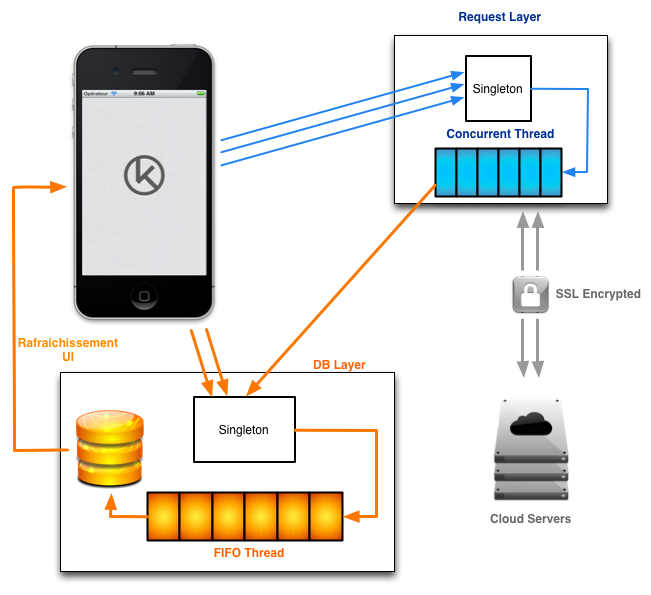
\includegraphics[width=400px]{Images/schema_general_simplifie.png}

Voici un plan général très synthétique du fonctionnement de notre application. Nous avons essayé de créer une architecture modulaire, utilisant une structure en couche permettant de s'adapter à l'ensemble des plateformes le plus simplement possible. Dans ce cas très précis, il me serait très simple de supprimer la partie interface graphique iPhone, mais de garder les moteurs pour les requêtes et la base de données afin de créer un client lourd pour OS X\footnote{OS X est le nom du système d'exploitation d'Apple, anciennement Mac OS puis Mac OS X} par exemple.\\

Chaque plateforme possède donc un langage spécifique (l'Objective-C et Cocoa pour Apple) et si nous connaissons les grands aspects et concepts de la programmation, il m'a fallu apprendre les spécificités de ce langage. Nous pouvons dégager trois grands aspects qu'il m'a fallu maîtriser dans le cadre de ce projet : 


\begin{itemize}
	\item Les requêtes au serveur (Request Layer sur le schéma)
	\item La base de données (DB Layer sur le Schéma)
	\item L'interface Graphique\\
\end{itemize}
Nous passerons un peu de temps à expliquer la complexité de chacune des parties citées ci-dessus.
		\paragraph{Les requêtes au serveur :}
		Cette partie a certainement été la moins complexe dans sa réalisation mais pour autant celle qui a  reçue le plus de modifications. Le premier système de requêtes en place était fonctionnel, mais le moindre changement à effectuer était un véritable cauchemar. Après de nombreuses manipulations, j'ai donc décidé de le changer entièrement dans sa structure. Nous pouvons donc retrouver actuellement une majeure partie du code écrit en premier lieu, mais son utilisation en est grandement simplifiée aujourd'hui.\\
		
		L'un des plus gros changements est survenu lorsque j'ai dû programmer le reprise de requêtes. Dans un environnement aussi mobile, nous travaillons énormément avec le serveur. Cependant, que se passe-t-il quand aucun réseau n'est disponible ? Certaines requêtes doivent-être sauvegardées, d'autres mises de côté pendant un certain temps. Devons-nous les enregistrer en base de données ? Quelle est la durée de vie de ces requêtes, et comment le savoir ? Nous sommes parvenus à un système pour l'ensemble de l'application où nous traitons avec des objets génériques possédants pouvant être sauvegardé en BD. Selon le type de requête, sa durée de vie est changée accordement (au moment ou l'application est tuée, ou quand l'utilisateur se délogue, etc.)  	\\
		
		C'est dans ce cas très précis que nous pouvons voir l'importance des projets d'urbanisation que nous avions lors de notre quatrième année. Au début du projet, puisque nous n'avions fait ni conception générale, ni de conception détaillée, nous nous sommes lancés dans un code peu propre, non maintenable, et peu enclin aux changements. Je pense qu'il est cependant impossible de se rendre compte de l'importance d'une bonne conception sans s'être une fois confronté au problème. \\
		
		C'est donc précisément ce pourquoi il est indispensable de porter un regard critique sur notre formation et ce genre de projet est indispensable pour le faire. Je me souviens d'une conversation en fin de troisième année avec un quatrième année qui m'a dit : "tu seras changé en fin de quatrième année, tu ne t'en apercevras pas tout au long, mais si tu compares tes aptitudes à travailler entre le début et la fin, tu verras l'importante évolution". Et il avait raison.\\
				
		\paragraph{La base de données :}
		Les bases de données sont un moyen efficace et simple à mettre en oeuvre afin de sauvegarder des informations de manière statique. Une première approche aurait donc été de reprendre une base dite classique avec l'approche que nous avions vue en cours (i.e. couche orientée services métiers, etc.). Ce n'est cependant pas le cas ici.\\
			
		Toujours dans une volonté d'apprendre ce langage, j'ai décidé d'utiliser Coredata, qui est l'outil de prédilection d'Apple pour les bases de données. Coredata est une surcouche logicielle pour les bases de données et permet une sérialisation immédiate des objets vers la base. Cette simplification a été dans un premier temps un vrai casse-tête, tellement la logique est différente de celle d'une base normale. \\
		
		Malheureusement, en raison de l'architecture de notre application, mais également de la faible quantité de mémoire à notre disposition dans les téléphones, attaquer les données depuis le thread principal (celui de l'interface) amène à une faible expérience utilisateur, l'interface étant lente, voir bloquée. C'est donc naturellement que je me suis tourné vers le multi-thread pour m'occuper de cela. Il m'a fallu près de six mois pour trouver les paramètres optimaux afin de pouvoir utiliser Coredata correctement, en raison de la concurrence d'accès aux données, donnant de temps à autre des données incohérentes, ou pire faisant crasher l'application.\\
		
		Nous apprenons le multitâche en troisième année ainsi que les problèmes de synchronisation, mais nous sortions ici des sentiers battus. Bien qu'il soit une surcouche C, l'objective-C reste un langage orienté objet, possédant ainsi ses propres implémentations des réponses classiques aux problèmes de synchronisation multi-thread. Il a fallu dans un premier temps rechercher les documentations et les forums, mais cette solution est vaine et parfois fortement trompeuse. Les réponses étaient cachées dans de nombreuses documentations, ce qui m'a fortement rappelé ces TPs d'architecture 3IF ! La base de données fonctionne désormais parfaitement.\\
		
		\paragraph{L'interface Graphique :}
		L'interface graphique a de tout temps été ce que j'aimais le moins mais cet élément est cependant indispensable puisque sans elle, l'utilisateur ne pourrait interagir avec le programme ! Il est tout à fait envisageable de réaliser une interface non complexe, et c'est ce qui a été fait dans un premier temps. Cependant, nous souhaitions, dans un souci de simplification d'utilisation pour l'utilisateur final, reprendre entièrement l'interface de l'application des SMS de la plateforme sur laquelle nous nous trouvions. Ceci représente un challenge de taille puisqu'Apple est réellement maniaque à ce niveau là. \\
		
		Nous avons cependant aujourd'hui une interface réellement identique, et quand j'utilise l'un des deux services (SMS ou Klaim) il m'est difficile de savoir quelle application je suis en train d'utiliser. Ce travail a été principalement réalisé par Quentin.\\
		
\subsubsection{La problématique du développement multiplateforme}
		Ceci est l'un des points les plus importants du document, puisqu'il parle d'un problème d'envergure dans le monde de l'informatique d'aujourd'hui. De plus en plus de personnes possèdent des Smartphones et les développeurs souhaitent donc développer des applications pour chacune des plateformes, mais cela demande énormément de temps et de connaissances. Si je suis capable aujourd'hui de créer une application pour iOS, je serais incapable de développer pour Androïd sans me plonger dans la documentation et de nombreux tutoriels. \\
		
		C'est pour cette raison que nous étions autant de monde sur le projet. Il y avait initialement deux personnes par plateforme afin de combler le manque de connaissances que nous avions.  C'est aujourd'hui l'une des plus grandes problématiques du moment avec la poussée de téléphones mobiles au sein de la société. \\
		
		Devant ce problème, des solutions ont été développées mais posent encore certains ennuis : 
		\begin{itemize}
			\item Réaliser un site web mobile permet de réduire considérablement le développement puisque les technologies à utiliser sont connues et nous n'avons qu'un seul code à écrire pour l'ensemble des plateformes. Cependant, nous ne pouvons rien sauvegarder sur la mémoire interne du téléphone ce qui peut être réellement problématique et critique selon le type d'applications que nous souhaitons développer, et nous n'avons surtout pas accès aux notifications, ces messages permettant d'indiquer à l'utilisateur un évènement particulier. 
			\item Il existe aujourd'hui des Framework permettant de réduire la charge de travail mais le résultat obtenu n'est pas aussi satisfaisant que celui d'une application dite native.\\
		\end{itemize}
		
		L'AEDI\footnote{l'Association des Etudiants du Département Informatique} organise régulièrement des conférences thématiques où des entreprises se déplacent pour nous parler d'un sujet particulier. C'est à cette occasion qu'une entreprise est venue nous parler de ce problème particulier, et ils font face aux mêmes interrogations que nous. J'en ai donc profité pour aller leur parler à la fin de la réunion et leur poser quelques questions. Leur avis a été le même que le nôtre : dans notre contexte, nous n'avons d'autre moyen que du développement natif pour une expérience utilisateur maximale, ce qui signifie donc du développement compliqué et des équipes spécifiques pour cela.
		
\subsubsection{Un cahier des charges évoluant constamment}
		Un autre souci important auquel nous avons été confronté initialement était le manque d'information sur ce que nous devions faire. Nous connaissions les idées directrices mais c'était tout. Nous apprenons lors de nos projets en école qu'il est important de bien étudier l'ensemble du projet afin de réaliser une conception répondant à toutes les exigences fonctionnelles comme non fonctionnelles. Une simple modification peut avoir d'importantes répercutions. \\
			
		C'est exactement l'inconvénient que nous avons eu pour diverses raisons. Premièrement parce que nous avons eu de nombreux problèmes auxquels il a fallu trouver une solution. Ces dernières apportaient parfois les modifications dont nous parlions précédemment. Deuxièmement car nous n'avons pas réellement effectué de conception générale pour l'ensemble du projet. Nous demandions uniquement à Quentin quelle était l'étape suivante une fois que nous avions terminé une partie. Cette façon de faire a posé de nombreux soucis et nous avons dû constamment apporter des changements à ce qui avait déjà été fait.\\
		
		Il aurait fallu idéalement que nous travaillions tous sur le cahier des charges, afin de l'étudier correctement, en relevant les besoins de l'ensemble du groupe. Bien que notre projet se décompose en sous-projets ayant cependant le même but, nous aurions pu faire une conception générale simplifiant ainsi la vie de l'ensemble des équipes. Au lieu de ça, nous nous sommes tous lancés dans notre architecture, ayant tous des problèmes (qui pour la plupart du temps, étaient identiques mais à des moments différents). Toutes les plateformes ont aujourd'hui une conception qui se ressemble, mais nous aurions gagné énormément de temps et d'énergie si elle avait été faite initialement. \\
		
		Lors de l'un des premiers projets de quatrième année ("DevOO"), nous nous sommes confrontés à un problème similaire. C'était le premier projet de programmation en hexanome, et il a fallu gérer l'ensemble du groupe, répartir les tâches à réaliser, obtenir une conception générale détaillée. Cela a été fait correctement mais malgré cela nous avons été en retard et il a fallu travailler la nuit pour finir le projet. Nous travaillions cependant sur le même projet tous ensemble, à l'inverse de Klaim où chaque plateforme était un projet à part entière. \\
		
	\subsection{Les problèmes liés au management de l'équipe}

	Nous avons principalement parlé des problèmes techniques, mais une grosse partie des dysfonctionnements auxquels nous avons été confrontés était liés à notre inexpérience dans la gestion d'équipe et de projet. Nous allons développer ceci dans la partie suivante. 
	
		\subsubsection{Une avancée difficile}
		Le principe du fil rouge est de supprimer un TP pour nous dégager du temps soit pour découvrir de nouvelles technologies soit pour développer des connaissances dans un domaine particulier. En ce sens, le projet fil rouge ne devrait pas en théorie dépasser une cinquantaine d'heure par personne, mais dans la réalité ce n'est pas ce qu'il se passe. D'autant plus qu'il est commun de ne voir que quelques personnes travailler réellement sur le projet. \\
		
		Dans notre cas, nous avions en quelque sorte 5 "fil rouge" à mener de face, ce qui a grandement complexifié la situation. Nous restons des étudiants et il a fallu jongler entre les projets d'école et Klaim, ce qui n'a pas été chose aisée. La majeure partie de nos week-end était consacrée à notre système de messagerie, et nous travaillions régulièrement chez moi les samedis. Malgré cela, nous n'avancions que très peu.\\ 
		
		Quand nous décidions d'instaurer quelques jalons afin de se motiver, nous tombions sur des difficultés plus importantes que nous devions régler en priorité. Il n'y avait donc pas de réelle satisfaction, tellement la fin semblait loin. Lors de la présentation en amphi du projet, nous n'avons même pas pu montrer un produit BlackBerry assez concluant, et au lieu de ça nous avons expliqué pourquoi il était aussi compliqué et peu agréable de travailler sur cette plateforme ! \\
		
		\subsubsection{Peu de connaissance en la matière}
		Un autre but du fil rouge est de montrer la difficulté du travail en groupe, mais notre éclatement en sous-projets a en réalité empêché cela. Plus grave encore, nous travaillions principalement en binôme, ce qui fait que nous n'avions pas de réel regard sur le travail des autres, et leur avancement. Ce dernier point était plus ennuyeux, puisque nous aurions pu en réalité tirer parti d'une compétition interne. Au lieu de ça, nous avancions un peu dans le flou, et nous nous sentions donc un peu seuls.\\
		
		Ce projet a essentiellement montré nos faiblesses dans la gestion d'équipe, quel que soit le nombre de personnes dans un projet, et notre besoin d'apprendre à gérer le temps, le stress et les collaborateurs. Le rôle du chef d'équipe était ici plus qu'important, afin de motiver l'ensemble des binômes, de tenir à jour un planning des tâches faites et à faire, et de donner des directives claires. Nous n'avons pas eu cette chance, et aucun de nous ne s'est d'ailleurs proposé pour le faire. \\
		
		C'est une des raisons pour laquelle j'étais impatient de me confronter à la quatrième année. Non seulement je voulais montrer aux promotions précédentes que ce n'était pas aussi dur que ce qu'ils disaient (j'avais tort !), mais également et surtout afin d'obtenir ces compétences qui me paraissent réellement importantes au sein d'un groupe. Avec le recul, aucun cours ne peut apprendre les bonnes pratiques pour cela, seul le fait d'être confronté aux problèmes en tant que chef de projet à travers des TPs permet de mieux appréhender ce qu'est réellement la gestion de projet.


\section{La gestion du temps et du projet}
		La quatrième année est centrée autour de la gestion de projet et d'équipe ; nous pouvons donc maintenant faire une analyse sur ce que nous avons appris.
		
	\subsection{Le temps, notre pire ennemi}
		\subsubsection{Un projet long à mener de front avec d'autres}
		Une autre problématique importante de Klaim était qu'il était extra-scolaire bien que dans le cadre du fil rouge. La troisième année reste une année chargée avec les projets et les examens de fin d'année et dans un cas comme le notre, le temps de programmation est très important. J'ai passé la majeure partie de mes week-ends à avancer sur le projet. J'aurai pu être bien plus efficace si j'avais connu le développement iOS avant mais ce n'était pas le cas.

		\subsubsection{L'écart des concurrents}
		Un aspect que nous n'avons pas encore réellement étudié dans ce document est la concurrence. Celle-ci existe déjà sur le marché et propose des produits fonctionnant très bien mais comme nous l'avons déjà énoncé, notre application possèdent quelques points pouvant réellement faire la différence.\\
		
		Commencer notre projet avec un tel retard est cependant dommageable puisqu'en attendant, le nombre de leurs clients augmente considérablement. Obtenir de nouveaux clients est bien plus facile que de détourner ceux qui utilisent un service identique.
		
	\subsection{Continuer le projet après la fin du fil rouge}
	Ce projet s'est commencé dans le cadre du fil rouge et après une présentation plus ou moins réussie, nous avions enfin terminé ! La pression allait enfin pouvoir retomber un peu après tant de travail, pour un résultat qui était prometteur mais encore peu concluant. Se posait alors la question "Qu'allons nous faire maintenant ?", qui était évidente pour certains mais beaucoup moins pour d'autres.


		\subsubsection{La démotivation au sein de l'équipe}
		L'avantage du projet scolaire facultatif nous libérant de la place sur notre plage horaire a été perdu à la fin des cours. Ce projet est devenu un fardeau pour certaines personnes du groupe puisque pour continuer, il fallait se remettre à travailler alors que les beaux jours arrivaient, et que la charge de travail pour les cours diminuait et que le stage allait commencer. \\
		
		Nous nous sommes donc réunis afin de demander qui était partant pour continuer, et toute l'équipe avait l'air favorable à cette idée. L'équipe BlackBerry a cependant cédé en premier annonçant qu'ils se confrontaient à trop de problèmes techniques, et que le projet n'était pas assez avancé malgré les efforts qu'ils avaient déjà déployés. Marc et Benjamin ont donc décidé d'arrêter. Ce fut le premier coup dur pour nous. L'autre Benjamin a également arrêté rapidement, n'arrivant pas réellement à travailler avec Quentin sur le site web. Nous n'étions donc plus que trois. \\
		
		Travailler à New York pendant mon stage, et essayer de rentrer le soir pour continuer le développement m'a demandé énormément de concentration et de volonté. J'ai cependant tenu le coup et continué d'avancer malgré moi. Je croyais au projet, et me disait que je ne pouvais pas réellement arrêter. En effet, j'étais le seul développeur iOS du moment, et bien que Quentin effectuait son stage sur cette plateforme, il n'avait pas le temps de supporter ce projet en plus. \\
	
		Alpha quant  à lui nous avait indiqué qu'il continuait de développer sur le projet. En réalité, ce n'était plus vraiment le cas et nous avons pris énormément de retard sur cette plateforme. A partir du mois d'août, nous n'étions plus que deux, et une motivation tombée bien bas, malgré un concept et des projets commençant à fonctionner correctement. \\
	
		Bref, mi-août, nous n'étions plus que deux. Quentin et moi. Comment continuer en partant d'ici ? J'avais toujours énormément de problèmes avec iOS, que je commençais cependant à mieux maîtriser. Quentin avait désormais le serveur, la version WP7\footnote{Windows Phone 7, système d'exploitation de Microsoft pour les téléphones mobiles} et le site web à gérer, sans parler de la plateforme Blackberry abandonnée. Nous avons cependant continué avec Quentin, car nous ne voulions pas avoir fait tout cela pour rien.\\
		
		Nous avons cependant réussi à trouver des personnes motivées début septembre pour reprendre le développement Android. 

		\subsubsection{Près d'un an sans release}
		L'un des principes que l'on tente de nous apprendre dans notre formation, est celui des jalons. Il est important de définir des objectifs pour un version d'un produit, et d'avoir une date butoir et de s'y tenir. Notre problème est que nous n'avons jamais eu de jalons bien défini, et nous avancions un peu comme nous pouvions, au fil de l'eau avec le temps qui nous restait en dehors des cours et des projets.  \\
		
		Le site a été lancé avec l'application WP7 en novembre, ce qui définissait un premier jalon important à nos yeux, puisqu'il représentait bientôt un an de travail. Bien que ce soit Quentin le responsable de ces deux plateformes, leur lancement m'a donné un coup de fouet pour continuer. Nous venions également de trouver deux personnes supplémentaires pour reprendre le projet Android, ce qui nous déchargeait d'un poids important !\\
		
		Je n'avais maintenant plus qu'à terminer l'application pour iOS. Elle était un peu plus stable, mais les graphismes n'étaient pas encore terminés, et de nombreux crash surgissaient encore, sans compter les manquements aux spécifications. Il y avait encore énormément de travail, et la quatrième année au département nous laissait vraiment trop peu de temps, d'autant plus que je m'occupais des relations entreprises pour l'AEDI, et des RIFs\footnote{les Rencontres IF est une journée où une trentaine d'entreprises se déplacent dans les locaux du département informatique afin de rencontrer les étudiants}. \\
		
		Au moment de l'écriture de ces lignes, l'application pour iOS est en cours de validation chez Apple et nous attendons leurs retours. Suite à la publication de cette version, nous allons pouvoir commencer à développer la version 2, puisqu'il y a énormément d'améliorations que nous voulons apporter afin de réduire l'écart avec nos concurrents. 
		
	\subsection{Les outils mis en place}
	En un an, nous avons utilisés différents outils, aussi bien pour le management des équipes, que pour la gestion des lignes de code, ce qui est absolument essentiel chez nous. Je vais en parler dans cette section, puisque c'est ce que nous avons appris cette année à réaliser. Nous utilisions donc déjà les moyens, sans avoir pour autant connaissance de leur potentiel ni de leur importance.
		\subsubsection{Les outils de code}
		Rapidement, nous nous sommes rendu compte qu'il serait important d'utiliser des outils afin de nous aider à nous guider ou travailler en groupe. Voici une liste des outils que nous avons utilisés (et que nous utilisons encore pour certains) :
			\begin{itemize}
				\item SVN : Subversion est un outil permettant de travailler collaborativement sur un projet. Il permet en plus de versionner le projet c'est-à-dire journaliser l'ensemble du code écrit, ce qui est d'autant plus important lorsque nous travaillons à plusieurs. Nous n'utilisons cependant plus ce service à ce jour.
				\item GIT : C'est le remplaçant pour nous de SVN qui propose certains avantages par rapport à SVN.
				\item Github : Héberger un serveur permettant d'utiliser GIT peut être contraignant. C'est pourquoi nous utilisons Github qui nous met des serveurs à disposition.
			\end{itemize}
		
\subsubsection{Les outils de management}
		Les outils cités ci-dessus permettent uniquement d'améliorer la vie des développeurs. Afin de gérer un projet informatique de cette envergure, il faut cependant bien plus. C'est pourquoi nous utilisons les outils suivants : 
		\begin{itemize}
			\item Redmine : est un outil de gestion de projet en ligne que nous utilisons depuis le début. Il permet de déclarer des projets et sous-projets, mais également de découper ces derniers en tâches et sous-tâches afin de les assigner à des ressources. Il est en quelque sorte une version webisée de Microsoft Project, mais avec des fonctionnalités cependant moins avancées. Cela nous permet cependant de suivre l'avancement des travaux de façon claire et précise.
			\item Klaim : maintenant que notre projet est assez avancé, nous l'utilisons énormément entre nous afin de nous donner des informations que nous voulons faire passer (i.e. petits bugs détectés ne demandant par forcément l'ouverture d'un ticket sous redmine).
			\item Jabbr : c'est un outil en ligne nous permettant de communiquer avec l'ensemble de l'équipe. Chaque personne peut voir ce que nous avons écrit et nous pouvons également consulter l'historique. Cela permet d'apporter de la connaissance générale sur l'ensemble des sous-projets. C'est une sorte de chat un peu comme IRC.
		\end{itemize}

\section{Vers l'infini et au delà}

	Notre désir de continuer le projet après la fin du fil rouge nous amène à encore travailler énormément dessus. Nous sommes actuellement quatre développeurs mais il nous faudrait idéalement bien plus de personnes. Après l'intégration de deux autres développeurs, nous avons un peu remanié notre organisation.

	\subsection{L'équipe actuelle}
	Avec le temps, je me suis aperçu que Quentin était un excellent développeur, cependant l'aspect de gestion de projet et de gestion des équipes ne l'intéressait absolument pas. N'étant plus que deux pendant l'été, cela ne posait pas réellement de problèmes. Cependant, avec l'arrivée de nouvelles personnes dans l'équipe, j'ai proposé de m'occuper de ce poste, ce à quoi Quentin avait l'air favorable. 
	\subsection{L'avancement du projet}
	A l'heure de l'écriture de ce PPH, la version web et WP7 est déjà sur le marché. La version iPhone est en cours de validation pour apparaitre sur l'AppStore\footnote{L'AppStore est le nom du magasin virtuel d'Apple où l'on peut télécharger des applications pour son téléphone} et nous espérons que cette version sera le grand lancement de notre service. \\
	
	Le développement de la version Android ayant pris du retard, cette plateforme devrait apparaître sous peu, surtout qu'après le lancement de la version iPhone, nous attendons un réel essor du nombre d'utilisateurs, et nous ne voulons pas perdre ces clients potentiels. En effet, ayant déjà pour le moment perdu la version Blackberry, nous ne pouvons nous permettre d'oublier une plateforme supplémentaire, surtout lorsqu'elle est aussi utilisée qu'Android. \\
	
	En attendant que la version 1 soit disponible sur Android, nous allons activement spécifier les futures fonctionnalités de l'application. Cela inclura dans un premier temps l'envoi de messages à plusieurs personnes afin de pouvoir converser plus facilement en groupe, puis dans un deuxième temps, il sera intéressant de pouvoir inclure des médias tel que les images ou la voix dans les messages.  
	
	\subsection{Le devenir du projet}
	A l'heure actuelle, nous sommes extrêmement motivés et nous recevons de bons retours de la part des testeurs. Nous avons également montré l'application à quelques professionnels fortement intéressés par le projet et les remontées sont plus qu'encourageantes.  Nous avons cependant peur avec Quentin qu'avec le stage cet été et les départs à l'étranger en cinquième année, nous perdions nos développeurs Android. \\
	
	Comme tout projet, il inclut une charge financière non compressible et c'est pourquoi nous cherchons des fonds auprès de sociétés d'investissement - également appelés des Business Angels" ou encore des "incubateurs". Malheureusement, cette recherche n’est pas évidente, mais avec la sortie des applications, nous pensons qu’il sera plus simple de trouver de quoi nous financer.  
	
	
\section{Conclusion}

		Ce PPH a été écrit dans plusieurs buts : 
		\begin{itemize}
			\item Montrer dans un premier lieu notre inexpérience dans un projet d'aussi grande envergure, avec autant d'éléments à gérer, que ce soit au niveau de la gestion des ressources humaines, mais également de la conduite d'un projet.
			\item Porter un regard sur notre formation de quatrième année, fortement axée sur la gestion de projet. \\
		\end{itemize}
		
		Ce premier point a été largement ressenti tout au long de l'année dernière, d'autant plus que Quentin n'était pas réellement intéressé par cette gestion - c'est en tout cas ainsi que je le percevais. L'ensemble des modifications qui ont été effectuées au cahier des charges a été plus que préjudiciable sur la date de rendu de projet. Nous ne pouvions malheureusement pas imaginer de façon claire et précise ce dans quoi nous nous jetions. C'est pour moi à ce jour le projet qui m'a fait acquérir le plus de compétences aussi bien dans le domaine technique, que dans le domaine des relations humaines, puisqu'il a fallu apprendre à communiquer au sein de notre groupe, bien que nous fussions des amis. \\
		
		La quatrième année au sein du département informatique est réputée pour être exigeante, aussi bien  pour l'ensemble de projets qu'il nous est demandé de rendre, et incidemment pour la charge de travail induite mais également car elle nous confronte étrangement à l'ensemble des problèmes que nous avons eus avec Klaim puisqu'il fallait gérer une équipe de six personnes (un hexanome) pour chaque projet. Il y avait cependant deux différences notables :
			\begin{itemize}
				\item Premièrement, chaque personne travaillait sur le même projet, et il était donc plus facile de contrôler l'avancement de chaque personne. 
				\item Deuxièmement, ces projets étaient dans le cadre des études, et nous étions donc "obligés" de les réaliser.\\
			\end{itemize}
		
		Il est possible que mon approche des projets en groupe était déjà différente en début de cette année, mais je sais qu'elle a énormément évoluée en un an. C'est aussi pourquoi je m'occupe de la coordination des différentes équipes de Klaim à ce jour, puisqu'il est important de le faire, afin de ne pas s'éparpiller comme nous l'avons fait auparavant.\\
		
		Je pense donc qu'il aurait été plus qu'intéressant de voir comment nous nous en serions sorti avec nos connaissances actuelles. Ce projet reste bien entendu extra-scolaire d'où la difficulté de l'avancer aussi vite que nous le souhaitons, mais c'est avec plaisir que nous continuons son développement. Nous sommes actuellement à la rechercher de fonds ainsi que de ressources humaines, mais nous avons les idées ainsi que le potentiel requis, et nous nous battons pour avancer.
	
\newpage	
\section{Annexes}
	\begin{itemize}
		\item capture version iPhone
		\item capture version web
		\item capture version WP7
	\end{itemize}
\end{document}
